\documentclass[11pt]{beamer}
\usepackage[utf8]{inputenc}
\usepackage[T1]{fontenc}
\usepackage[francais]{babel}
\usepackage{amsmath}
\usepackage{amsfonts}
\usepackage{amssymb}
\usepackage{graphicx}
\usetheme{Montpellier}


\begin{document}
	\author{Mauricio Caceres}
	\title{Antennes Intelligentes}
	\subtitle{Methodes numeriques}
	\logo{}
	\institute{ENSSAT}
	\date{10 f2vrier 2017}
	\subject{Présentation travail autonomme}
%	\setbeamercovered{transparent}
	\setbeamertemplate{navigation symbols}{}
	\frame[plain]{\maketitle}
%---------------------------------------------------
%
%	INTRODUCTION
%
%---------------------------------------------------	
	\section{Introduction}
	\begin{frame}
	\subsection{One}
		\frametitle{}
	\end{frame}
%---------------------------------------------------
%
% CORP
%
%---------------------------------------------------

\begin{frame}
	\subsection{One}
	\frametitle{}
	
	\begin{figure}
\centering
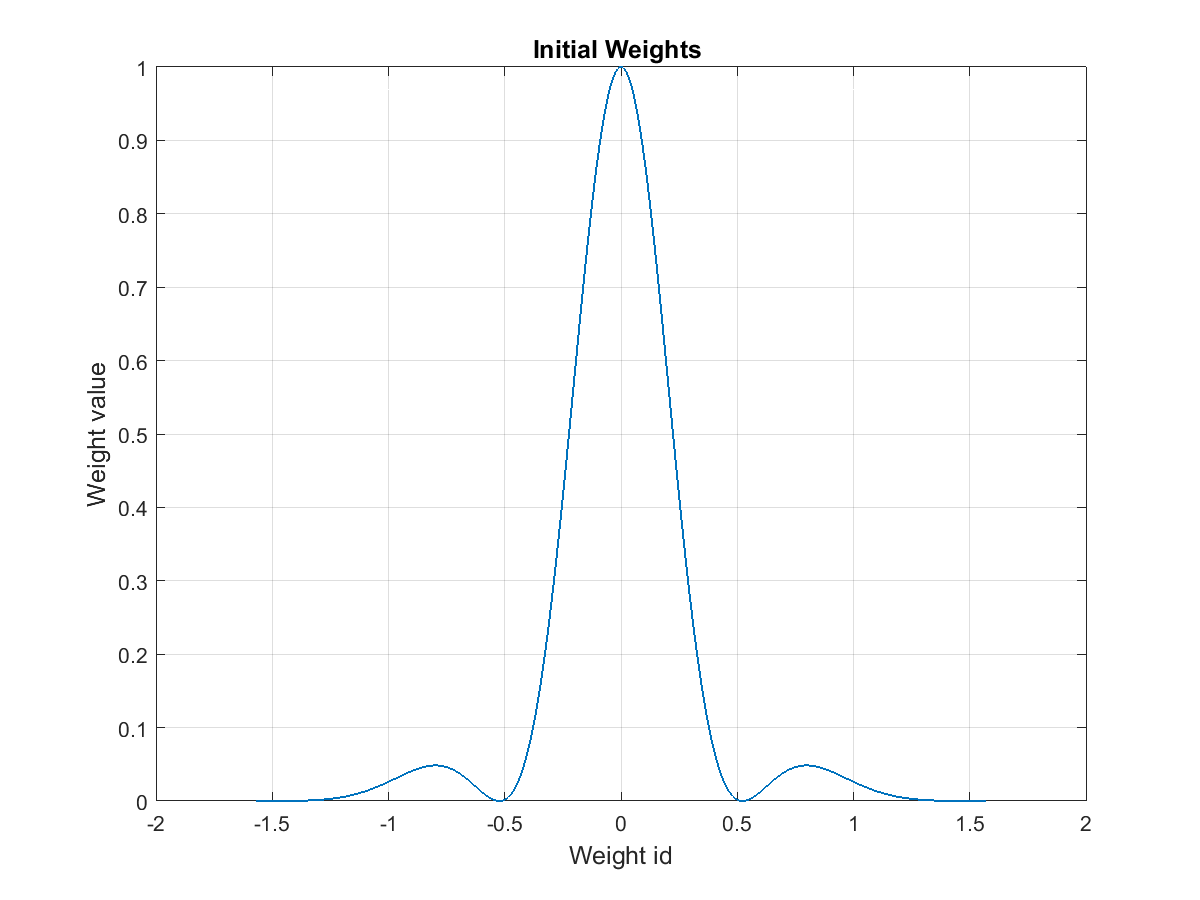
\includegraphics[width=0.3\linewidth]{../src/fiche1/exo2_1}
\caption{}
\label{fig:exo2_1}
\end{figure}

	
	
\end{frame}
%---------------------------------------------------

\begin{frame}
	\subsection{One}
	\frametitle{}
\end{frame}
%---------------------------------------------------

\begin{frame}
	\subsection{One}
	\frametitle{}
\end{frame}
%---------------------------------------------------

\section{Deuxième optimisation : le filtre à minimun de variance}
\begin{frame}
	\subsection{One}
	\frametitle{Deuxième optimisation : le filtre à minimun de variance}
%Considerations
%	\begin{itemize}
%		\item Même scénario précedent
%		\item Une source utile placée dans un angle $\phi_s$
%		\item Deux signaux interferentes $I_1$ et $I_2$ placées à $\phi_1$ et $\phi_2$.
%		\item signal reçu à chaque capteur est $x_m(n) = s_m(n) + i_m(n) + i_m(n) + b_m(n), m = 1,2, ... , M et \forall n \in N$
%	\end{itemize}
%	Considerations
% Même scénario précedent

% Une source utile placée dans un angle $\phi_s$
% Deux signaux interferentes $I_1$ et $I_2$ placées à $\phi_1$ et $\phi_2$.
% signal reçu à chaque capteur est $x_m(n) = s_m(n) + i_m(n) + i_m(n) + b_m(n), m = 1,2, ... , M et \forall n \in N$
	
\end{frame}
%---------------------------------------------------
\subsection{Exercise 4.1 : Problème d'optimisation}
\begin{frame}

	\frametitle{Solution problème d'optimisation}
\end{frame}
%---------------------------------------------------
	\subsection{Exercise 4.2 : Analyse }
	\begin{frame}
		
	
		\frametitle{Calcul de vecteur de ponderations optimales}
	\end{frame}
%---------------------------------------------------
	\begin{frame}

		\frametitle{Diagrammes}
	\end{frame}
%---------------------------------------------------
\begin{frame}
	
	\frametitle{Génération des signaux et diagramme de l'oeil}
\end{frame}
%---------------------------------------------------
\begin{frame}

	\frametitle{Simulations des autres scénarios}
\end{frame}
%---------------------------------------------------
\begin{frame}
	\subsection{One}
	\frametitle{}
\end{frame}
%---------------------------------------------------

\begin{frame}
	\subsection{One}
	\frametitle{}
\end{frame}
%---------------------------------------------------

\begin{frame}
	\subsection{One}
	\frametitle{}
\end{frame}
%---------------------------------------------------



\begin{frame}
	\subsection{One}
	\frametitle{}
\end{frame}
%---------------------------------------------------

\begin{frame}
	\subsection{One}
	\frametitle{}
\end{frame}
%---------------------------------------------------

\begin{frame}
	\subsection{One}
	\frametitle{}
\end{frame}
%---------------------------------------------------
%	FIN
%
%---------------------------------------------------
	\section{FIN}
\begin{frame}
	\subsection{One}
	\frametitle{}
\end{frame}
%---------------------------------------------------








\end{document}